\section{Modelo de datos de MongoDB}
\label{cap:mongodb}

MongoDB guarda los documentos originales de ListenBrainz en la colección \code{listens} de la base \code{listenbrainz_db} \citep{mongodb}. Es la base que conserva el dato tal como llegó: las otras dos transforman las escuchas en tablas agregadas o en relaciones, pero si hace falta volver a procesar un registro, el original está aquí. El código está en \code{databases/mongodb/}.

\subsection{Modelo documental}

Cada escucha es un documento. Se guarda con la misma estructura del volcado, sin renombrar ni aplanar campos, más un \code{_id}:

\begin{lstlisting}[language=JSON]
{
  "_id": "listenbrainz:<huella SHA-256 del documento>:1",
  "user_id": 12345,
  "user_name": "usuario_ejemplo",
  "timestamp": 1793318246,
  "recording_msid": "identificador-ejemplo",
  "track_metadata": {
    "track_name": "Cancion de ejemplo",
    "artist_name": "Artista de ejemplo",
    "release_name": "Album de ejemplo",
    "additional_info": {}
  }
}
\end{lstlisting}

Mantener el anidamiento de \code{track_metadata} tiene sentido porque esos campos describen la pista y se leen juntos, y porque \code{additional_info} cambia de un registro a otro según el cliente que envió la escucha: en un modelo de tablas habría que decidir de antemano qué columnas guardar y se perdería el resto. El \code{_id} de los documentos cargados desde el volcado se deriva de una huella SHA-256 del contenido, de modo que el mismo documento siempre recibe el mismo identificador. Los documentos creados a mano por el CRUD o la API reciben un \code{ObjectId} normal.

\subsection{Índices}

Se crean tres índices compuestos, pensados para las consultas que hace la aplicación (tabla~\ref{tab:mongo-indices}). Todos terminan en \code{_id} para que el orden sea total y la paginación por cursor sea estable aunque haya escuchas con la misma fecha.

\begin{table}[H]
\centering
\caption{Índices de la colección \code{listens}}
\label{tab:mongo-indices}
\begin{tabularx}{\textwidth}{l Y}
\toprule
Índice & Consulta que acelera \\
\midrule
\code{(timestamp -1, _id -1)} & Escuchas más recientes y paginación cronológica \\
\code{(user_name 1, timestamp -1, _id -1)} & Historial de un usuario, de la más reciente a la más antigua \\
\code{(track_metadata.artist_name 1, timestamp -1, _id -1)} & Escuchas de un artista ordenadas por fecha \\
\bottomrule
\end{tabularx}
\end{table}

La validación del módulo comprobó con \code{explain} que las tres consultas usan su índice (etapa \code{IXSCAN}) y que examinan exactamente los documentos que devuelven: por ejemplo, 20 claves examinadas para 20 resultados en la consulta cronológica, con un tiempo de ejecución de 1~ms sobre una colección de 4\,000\,001 documentos.

\subsection{Carga por lotes}

La carga masiva está en \code{databases/mongodb/loader.py}, cuya función \code{load_to_mongodb} llama al importador de \code{app/services/import_service.py}. El importador lee el archivo línea a línea y procesa cada registro así:

\begin{enumerate}
  \item Interpreta la línea como JSON y valida el documento con el modelo Pydantic \code{ListenCreate}: \code{user_name} con entre 1 y 1000 caracteres, \code{timestamp} entero dentro del rango de fechas válido, nombre de canción y de artista no vacíos y claves de metadatos que no empiecen con \code{$} ni contengan puntos, que MongoDB no admite. Las líneas inválidas se registran en un archivo de errores y se saltan.
  \item Calcula la huella SHA-256 del documento serializado con claves ordenadas y la compara con las huellas ya cargadas, que guarda en un SQLite auxiliar. Si ya existe, cuenta como duplicado y no se inserta.
  \item Agrupa los documentos nuevos en lotes (2000 por defecto, como máximo 5000) y los inserta con \code{insert_many(ordered=False)}. Si un documento ya estaba en la colección, el error de clave duplicada se ignora y el resto del lote se inserta igual.
  \item Después de cada lote guarda en el SQLite las huellas nuevas y el byte del archivo donde quedó la lectura (checkpoint).
\end{enumerate}

Gracias al checkpoint, una carga interrumpida continúa desde el último lote confirmado, y como las huellas se reconstruyen a partir de la colección al empezar, lo que alcanzó a insertarse antes de la interrupción no se duplica. Un archivo de bloqueo impide que dos cargas corran a la vez sobre el mismo estado. La función acepta un \code{limit} de documentos por ejecución y un tope total de 4\,000\,000 documentos en la colección.

Al integrar el módulo con Airflow corregimos el cálculo de ese tope. \code{load_to_mongodb} le pasaba \code{limit} como total objetivo de la colección, así que desde la segunda ejecución el objetivo ya estaba alcanzado y no se insertaba nada. Ahora el objetivo es la cantidad actual de documentos más \code{limit}, con el tope de 4\,000\,000, y cada ejecución agrega el siguiente bloque del archivo.

La validación del módulo se hizo sobre una colección de 4\,000\,001 documentos. La importación que la llenó procesó 4\,000\,000 de líneas en unos 5\,570 segundos: insertó 3\,950\,000 y marcó 50\,000 como duplicadas, que eran justamente los 50\,000 documentos ya cargados en una prueba anterior. Según su registro, esa carga se leyó del incremental 2754 (31 de octubre de 2026), un volcado posterior al que usa el resto del proyecto, por lo que sus resultados analíticos no se comparan directamente con los de Cassandra y Neo4j. En las corridas del DAG la colección se llena con el incremental 2746, igual que las otras dos bases (sección~\ref{sec:airflow-corridas}).

\subsection{Operaciones CRUD}

El script \code{python -m databases.mongodb.crud --pause} demuestra las cuatro operaciones con funciones de \code{databases/mongodb/crud.py}, deteniéndose entre pasos para explicarlas:

\begin{table}[H]
\centering
\caption{Operaciones CRUD en MongoDB}
\label{tab:mongo-crud}
\begin{tabularx}{\textwidth}{l l Y}
\toprule
Operación & Función & Operación en PyMongo \\
\midrule
Crear & \code{insert_listen} & \code{insert_one} con el documento de la escucha \\
Consultar & \code{get_listen}, \code{get_user_listens} & \code{find_one} por \code{_id}; \code{find} por usuario ordenado por fecha descendente \\
Actualizar & \code{update_listen} & \code{update_one} con \code{$set}, por ejemplo sobre \code{track_metadata.track_name} \\
Eliminar & \code{delete_listen} & \code{delete_one} por \code{_id} y comprobación de que ya no existe \\
\bottomrule
\end{tabularx}
\end{table}

La figura~\ref{fig:mongo-crud} muestra la demostración ejecutada sin pausas contra la colección que dejó Airflow. El documento de prueba usa un usuario ficticio y al final se borra, así que la colección queda con los mismos documentos.

\begin{figure}[H]
\caption{Demostración del CRUD en MongoDB}
\label{fig:mongo-crud}
\centering
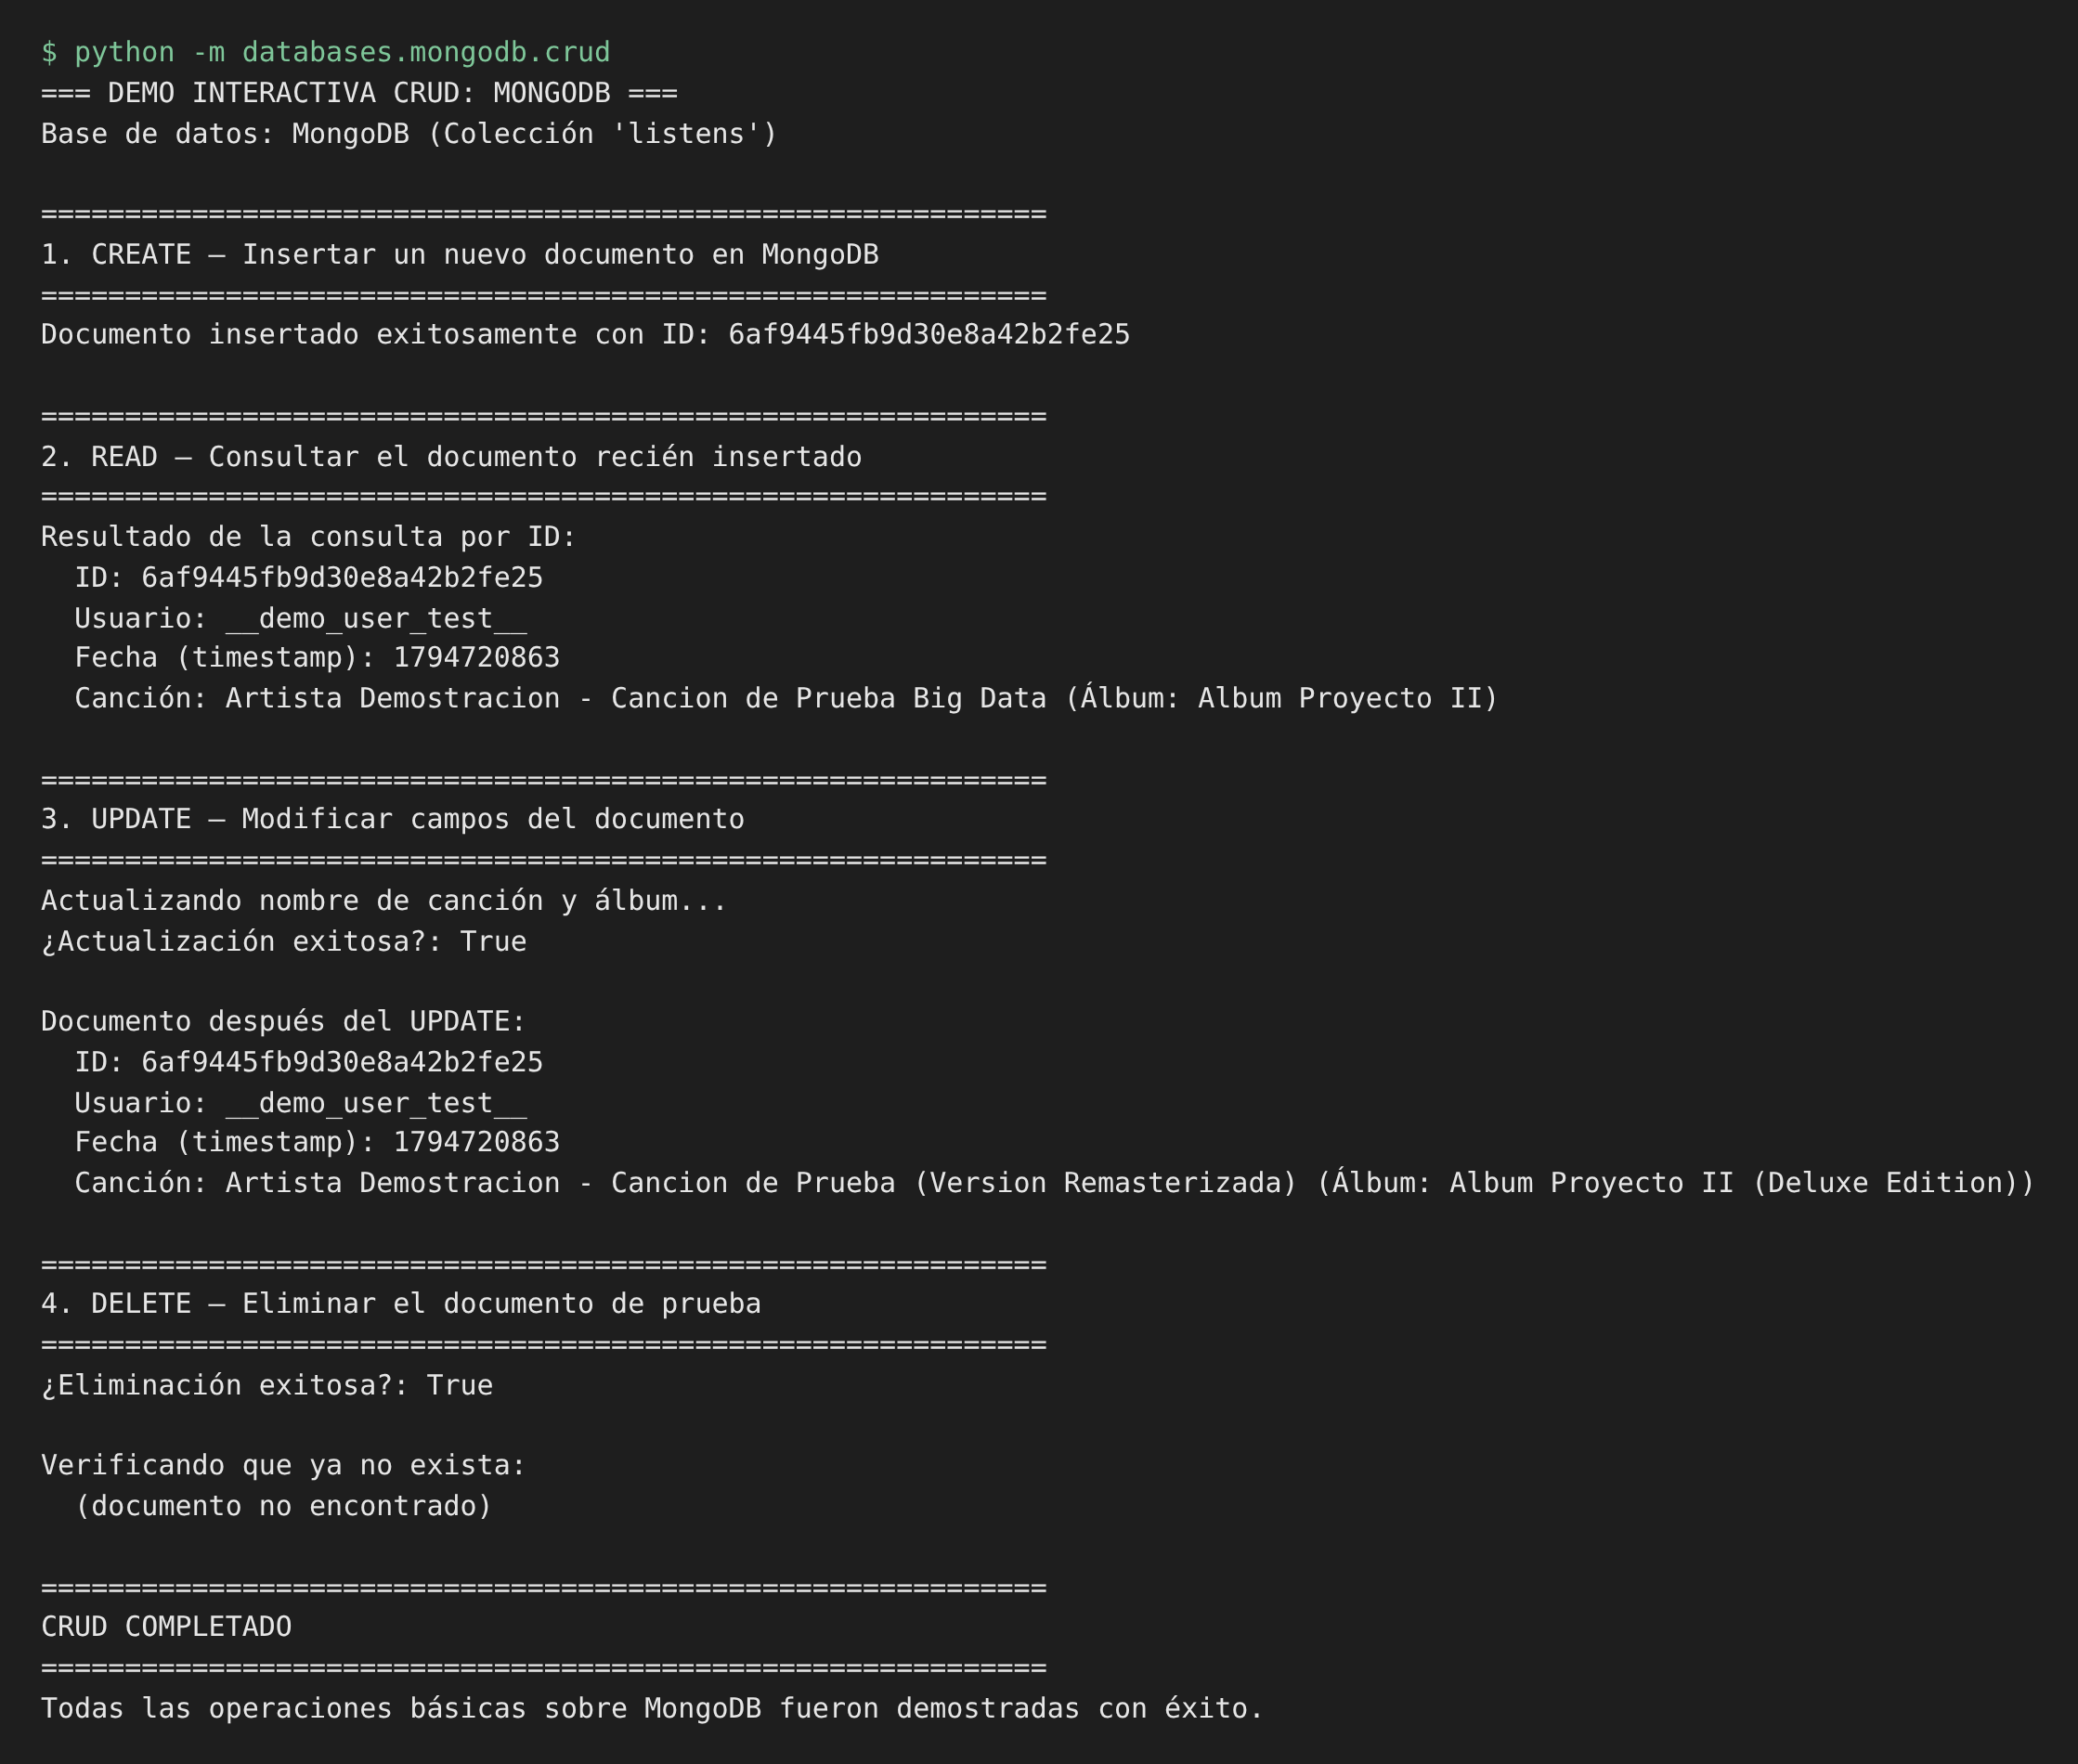
\includegraphics[width=\textwidth]{figuras/mongo_crud.png}
\end{figure}

El módulo incluye además una API REST con FastAPI sobre la misma colección, con documentación interactiva en Swagger. Las rutas bajo \code{/listens} cubren creación (\code{POST}), consulta por identificador y listado paginado (\code{GET}), actualización parcial y total (\code{PATCH} y \code{PUT}) y eliminación (\code{DELETE}), además de un resumen estadístico y un top de artistas. Cada solicitud pasa por la ruta, el modelo Pydantic que valida los campos (y responde 422 si son incorrectos antes de escribir en la base), un servicio que arma los filtros y un repositorio que ejecuta la operación con PyMongo. En la validación final se ejecutaron tres rondas completas de CRUD por HTTP contra la colección real y la cantidad de documentos quedó igual antes y después.

\subsection{Consultas y agregaciones}

\code{databases/mongodb/queries.py} define siete agregaciones: usuarios únicos, artistas únicos, top 5 de artistas, top 10 de canciones (agrupadas por artista y título), top 5 de usuarios, duración promedio de las pistas que traen \code{duration_ms} en \code{additional_info} y escuchas por día. La última convierte el \code{timestamp} a fecha y agrupa por día:

\begin{lstlisting}[language=Python]
"listens_by_day": [
    {"$match": {"timestamp": {"$type": "number", "$gte": 0, "$lte": 253402300799}}},
    {"$project": {"day": {"$dateToString": {"format": "%Y-%m-%d", "timezone": "UTC",
                  "date": {"$toDate": {"$multiply": ["$timestamp", 1000]}}}}}},
    {"$group": {"_id": "$day", "listen_count": {"$sum": 1}}},
    {"$sort": {"_id": 1}},
],
\end{lstlisting}

Estas agregaciones recorren la colección completa y sirven para exploración. Los indicadores que se consultan siempre, como las escuchas por día, se precalculan en Cassandra, que los sirve en milisegundos.

MongoDB guarda también la colección \code{kpi_runs}, donde Airflow deja un documento por corrida con los cinco KPIs, las métricas de seguimiento y la serie diaria reciente (sección~\ref{cap:kpis}).
